\documentclass[a4paper,12pt]{book}
\usepackage[utf8]{inputenc}
\title{}
\author{Rachel Morris}
\date{\today}

\usepackage{rachwidgets}
\usepackage{fancyhdr}
\usepackage{lastpage}
\usepackage{dirtree}
\usepackage{boxedminipage}

\newcommand{\laChapter}{5.1\ }

\pagestyle{fancy}
\fancyhf{}
\lhead{CS 211}
\chead{Fall 2017}
\rhead{Ch \laChapter Exercise}
\rfoot{\thepage\ of \pageref{LastPage}}
\lfoot{\scriptsize By Rachel Morris, last updated \today}

\renewcommand{\headrulewidth}{2pt}
\renewcommand{\footrulewidth}{1pt}

\begin{document}

    %\toggletrue{answerkey}
    \togglefalse{answerkey}

    %------------------------------------------------------------------%
    %- INSTRUCTIONS ---------------------------------------------------%
    %------------------------------------------------------------------%
    
    \chapter*{Chapter \laChapter In-class Exercise} \stepcounter{chapter}

    \iftoggle{answerkey}{
      \begin{answer} ANSWER KEY \end{answer}
    }{}
    
    \paragraph{Info:}
    In-class exercises are meant to introduce you to the new topics
    of this chapter of the book. Each part will have an introductory
    description of the content and example(s), followed by practice
    problems for you to work on. ~\\

    These assignments are \textbf{team assignments} - your team will
    turn in \textit{one} copy of the exericse. It is up to your team
    how to appropach the assignments; you can work separately and then
    check your work together, or you can collaborate on the assignment
    together. ~\\

    Work must be clean; points may be deducted if the instructor cannot
    read the work.

    \hrulefill{}
    
    \newpage{}

    %------------------------------------------------------------------%
    %- Exercise Begin -------------------------------------------------%
    %------------------------------------------------------------------%
    \begin{center} \section*{Chapter \laChapter In-class Exercise Instructions} \end{center}

    \begin{center}
        \textbf{This is the instruction page, 
        make sure to fill out your answers in the \textbf{worksheet} later in the document}
    \end{center}

    %------------------------------------------------------------------%
    \section*{1. Review: Sets}

        \begin{introNOHEAD}
            In CS 210, chapter 3, we worked with \textbf{sets} and their properties.
            When we work with finite sets, there is a limited amoutn of
            elements in the set, and it can be written out. ~\\

            Elements of a set are contained within curly braces \{ \},
            and are separated by commas. Example: $\{ 1, 2, 3 \}$. ~\\

            Additionally, repeated elements in a set does not make it
            unique from an otherwise same set without the duplicates.
            In other words, $\{1, 1, 2, 3, 5\}$ is the same as $\{1, 2, 3, 5\}$. ~\\

            Additionally, order is not important with sets.
        \end{introNOHEAD}

        % - QUESTION --------------------------------------------------%
        \begin{question}{1}{15\%}
            Given the \textbf{ Universal Set } $U = \{ 1, 2, 3, 4, 5, 6 \}$,
            write out the following subsets (on the worksheet):
        \end{question}

        \begin{enumerate}
            \item[a.] The subset of $U$ that contains all the even numbers.

            \item[b.] The subset of $U$ that contains all the prime numbers.

            \item[c.] The subset of $U$ that contains all the odd numbers less than 4.
        \end{enumerate}

    
    %------------------------------------------------------------------%
    \section*{2. Types of ordering}

        \begin{introNOHEAD}
            For some types of data, we care about the ordering, and for
            others, we do not. For example, with the above problems,
            we don't care about the order of numbers listed for our subsets.
            In other cases, we might care about the order of our elements.
            For this section, we will look at data and decide whether it
            should be in an \textbf{ordered list} or an \textbf{unordered list}.
        \end{introNOHEAD}

        % - QUESTION --------------------------------------------------%
        \begin{question}{2}{8\%}
            At The Ordered Cinema, customers are required to enter in
            their heights while buying tickets.
            In any given column of movie seats, customers must be seated
            according from shortest (in front, at the beginning of the set) to tallest (in back, at the end of the set).
            ~\\

            The heights of several patrons awaiting seating are: 
            $\{ 5'5'', 5'4'', 6'0'', 4'9'' \}$
            ~\\
            
            If there are only 2 seats available in each column,
                how many different ways could these customers be ordered in 2 seats?
                (Assume other customers will be seated in a different column.)
                ~\\
        \end{question}

        
        \begin{introNOHEAD}
            \paragraph{An ordered list}
                Is a finite list where sequence order matters.
            
            \paragraph{An unordered list}
                Is a finite list where sequence order does not matter.
        \end{introNOHEAD}

    
    %------------------------------------------------------------------%
    \section*{3. Combinations and Permutaions}

        \begin{introNOHEAD}
            \paragraph{Combination}
                In mathematics, a combination is a way of selecting items from a collection,
                such that (unlike permutations) the order of selection does not matter.
                \footnote{From https://en.wikipedia.org/wiki/Combination}
                
            \paragraph{Permutation}
                In mathematics, the notion of permutation relates to the act of arranging
                all the members of a set into some sequence or order, or if the set is already ordered,
                rearranging (reordering) its elements, a process called permuting. These differ from combinations,
                which are selections of some members of a set where order is disregarded. For example, written as tuples,
                there are six permutations of the set \{1,2,3\}, namely: (1,2,3), (1,3,2), (2,1,3), (2,3,1), (3,1,2), and
                (3,2,1).
                \footnote{From https://en.wikipedia.org/wiki/Permutation}
        \end{introNOHEAD}


        % - QUESTION --------------------------------------------------%
        \newpage
        \begin{question}{3}{23\%}
            Four students are buying folders from the campus bookstore,
            and each need three folders each for English, Discrete Structures,
            and Biology. Folders are available in different colors: white, green, red, and blue.
            Each student chooses their folders in different ways:
            \footnote{Question originally from Jim Van Horn's POGIL exercises}

            \begin{framed}
                \textbf{Uyriah:} Grabbed 3 folders without consideration for color.

                \hrulefill
                
                \textbf{Orlando:} Chose folders in order: First English, second Discrete Structures,
                and third Biology.

                \hrulefill

                \textbf{Connie:} Chose folders of 3 different colors, but doesn't matter which color
                for what class.

                \hrulefill

                \textbf{Pete:} Selected folders in order by class like Orlando, and chose separate
                colors for each like Connie.
            \end{framed}
        \end{question}

        \begin{enumerate}
            \item[a.] In this model, how many different colors were available at the bookstore?

            \item[b.] How many folders would each student choose?

            \item[c.] In the table below, indicate which student's selection corresponds with
                each of the two dimensions. (Put the student's initial in the table on the worksheet.)

                \begin{tabular}{ | l | c | p{2cm} | p{2cm} | }
                    \hline
                    & & \multicolumn{2}{ r | }{ Did the order of selection matter? }
                    \\ \hline{}
                    & & YES & NO
                    \\ \hline

                    \multirow{2}{*}{ Was color repetition allowed? } & YES & & \\\cline{2-4}
                        & NO & &
                    \\ \hline 
                \end{tabular}

            \item[d.] For which students were repeating colors acceptable?
            
            \item[e.] For which students were repeating colors \textit{not} acceptable?

            \item[f.] Which students' selections would be an \textit{ordered list}?

            \item[g.] Which students' selections would be an \textit{unordered list}?
        \end{enumerate}

        \newpage
        These types of sequences where repetition is not allowed are known are called
        \textbf{permutations} and \textbf{combinations}.
        For permutations the order is important.

        \begin{enumerate}
            \item[h.] Which student’s selections demonstrate a permutations?

            \item[i.] Which student's selections demonstrate a combination?
        \end{enumerate}

        \begin{hint}{Hint:}
            These student names correspond with the representations...
            \underline{U}nordered, \underline{O}rdered, \underline{P}ermutation,
            and \underline{C}ombination.            
        \end{hint}


        \hrulefill

        \begin{introNOHEAD}
            When we're flipping a coin, there are two possible outcomes:
            \textit{heads} or \textit{tails}. If we flip more than one
            coin, then we end up with more possible outcomes. For example,
            when flipping two coins, we have four possible outcomes:

            \begin{center}
                \begin{tabular}{ | l | c | c | }
                    \hline
                    & First coin & Second coin \\ \hline
                    1. & HEADS & HEADS \\ \hline
                    2. & HEADS & TAILS \\ \hline
                    3. & TAILS & HEADS \\ \hline
                    4. & TAILS & TAILS \\ \hline
                \end{tabular}
            \end{center}

            In this case, order matters and (H,T) is a different result
            from (T,H).
        \end{introNOHEAD}
        
        % - QUESTION --------------------------------------------------%
        \begin{question}{4}{14\%}

            We have a pool of four people, \{Andrew, Bob, Carly, Diane\}, and two prizes will be distributed
            between two of these people.
            \footnote{Based on Practice Problem 2 from Discrete Mathematics, Ensley \& Crawley}

            \begin{enumerate}
                \item[a.] Assuming that prize \#1 and prize \#2 are different, list out
                all the ways the prizes can be distributed (i.e., permutations).

                \textit{Example: (A, A), (A, B), (B, A), ...}

                \item[b.] Assuming that prize \#1 and price \#2 are both the same,
                list out all the ways the prizes can be distributed (i.e., sets).

                \textit{Note: \{A, B\} and \{B, A\} would be considered the same.}
            \end{enumerate}
            
        \end{question}
        
        % - QUESTION --------------------------------------------------%
        \begin{question}{5}{20\%}

            All possible outcomes of rolling a red 6-sided die and a green 6-sided die,
            in an organized way: ~\\

            \begin{tabular}{ l | l l l l l l }
                & Green 1 & Green 2 & Green 3 & Green 4 & Green 5 & Green 6 \\ \hline
                Red 1 & (1,1) & (1,2) & (1,3) & (1,4) & (1,5) & (1,6) \\
                Red 2 & (2,1) & (2,2) & (2,3) & (2,4) & (2,5) & (2,6) \\
                Red 3 & (3,1) & (3,2) & (3,3) & (3,4) & (3,5) & (3,6) \\
                Red 4 & (4,1) & (4,2) & (4,3) & (4,4) & (4,5) & (4,6) \\
                Red 5 & (5,1) & (5,2) & (5,3) & (5,4) & (5,5) & (5,6) \\
                Red 6 & (6,1) & (6,2) & (6,3) & (6,4) & (6,5) & (6,6) \\
                
            \end{tabular}
            ~\\

            For the given set of data, answer the questions.
            \footnote{Based on Exercise 5.1 \#6 from Discrete Mathematics, Ensley \& Crawley}

            \begin{enumerate}
                \item[a.]   Of the listed outcomes, how many are ``doubles"
                            (both dice have the same value)? What percentage of
                            total outcomes does this represent?
                            (You can write it as a fraction)

                \item[b.]   How many are doubles \textit{and} have the sum
                            of two dice values less than 4?
                            (You can write it as a fraction)

                \item[c.]   How many have a 5 on exactly one of the dice?

                \item[d.]   How many have a 5 on at least one of the dice?
            \end{enumerate}
            
        \end{question}
                
        % - QUESTION --------------------------------------------------%
        \newpage
        \begin{question}{6}{20\%}

            The following tree lists all possible outcomes of tossing a penny,
            a nickel, and a dime together:

            \begin{center}
                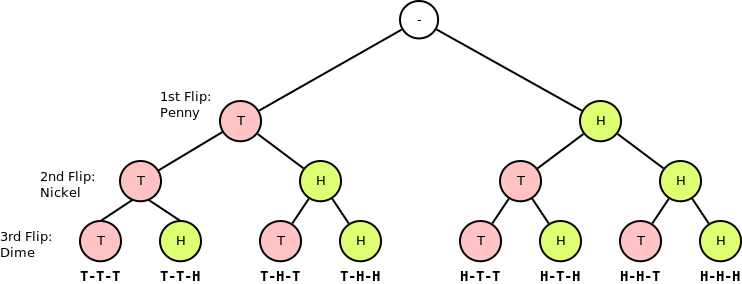
\includegraphics[width=13cm]{images/5-1-gametree.png}
            \end{center}

            For the given set of data, answer the questions.
            \footnote{Based on Exercise 5.1 \#8 from Discrete Mathematics, Ensley \& Crawley}

            \begin{enumerate}
                \item[a.] Of the outcomes shown, for how many does
                the result on the penny match the result on the dime?

                \item[b.] Which is more likely, that the result on the penny
                matches the result on the dime, or that they do not match?

                \item[c.] For how many of the outcomes do all three coins match?

                \item[d.] For how many of the outcomes do exactly two of the coins match?

                \item[e.] For how many outcomes is the number of tails less than the number of heads?
            \end{enumerate}
            
        \end{question}
        
    %------------------------------------------------------------------%
    %- Exercise Begin -------------------------------------------------%
    %------------------------------------------------------------------%

    %------------------------------------------------------------------%
    \newpage{}
    \section*{Answer sheet}

    ~\\
    % - QUESTION --------------------------------------------------%
    \begin{answersheetquestion}{1}{Subsets of $U = \{ 1, 2, 3, 4, 5, 6 \}$}{15}

        \begin{enumerate}
            \item[a.] The subset of $U$ that contains all the even numbers. ~\\
                \iftoggle{answerkey}{ \begin{answer}
                    $\{ 2, 4, 6 \}$
                \end{answer} }{}

            \item[b.] The subset of $U$ that contains all the prime numbers.  ~\\
                \iftoggle{answerkey}{ \begin{answer}
                    $\{ 1, 2, 3, 5 \}$
                \end{answer} }{}

            \item[c.] The subset of $U$ that contains all the odd numbers less than 4.  ~\\
                \iftoggle{answerkey}{ \begin{answer}
                    $\{ 1, 3 \}$
                \end{answer} }{}
        \end{enumerate}
        
        
    \end{answersheetquestion}

    ~\\
    
    \hrulefill
    
    ~\\
    % - QUESTION --------------------------------------------------%
    \begin{answersheetquestion}{2}{Movie seating}{8}
        List all combinations for any 2 customers, make sure
                shorter people come before taller people.
                \iftoggle{answerkey}{ \begin{answer}
                        $\{ 4'9'', 5'4'' \}$ \tab
                        $\{ 4'9'', 5'5'' \}$ \tab
                        $\{ 4'9'', 6'0'' \}$ \\
                        $\{ 5'4'', 5'5'' \}$ \tab
                        $\{ 5'5'', 6'0'' \}$ \tab
                \end{answer} }{ { ~\\ \raisebox{0pt}[2cm][0pt]{  } } }
        
    \end{answersheetquestion}
    ~\\
    
    \hrulefill{}

    
    ~\\
    % - QUESTION --------------------------------------------------%
    \newpage
    \begin{answersheetquestion}{3}{Student folders}{23}
       
        \begin{enumerate}
            \item[a.] In this model, how many different colors were available at the bookstore?
                \iftoggle{answerkey}{ \begin{answer} 4 \end{answer} }{}

            \item[b.] How many folders would each student choose?
                \iftoggle{answerkey}{ \begin{answer} 3 \end{answer} }{}

            \item[c.] In the table below, indicate which student's selection corresponds with
                each of the two dimensions. (Put the student's initial in the table on the worksheet.)

                \begin{tabular}{ | l | c | p{2cm} | p{2cm} | }
                    \hline
                    & & \multicolumn{2}{ r | }{ Did the order of selection matter? }
                    \\ \hline{}
                    & & YES & NO
                    \\ \hline

                    \multirow{2}{*}{ Was color repetition allowed? } & YES
                        & \iftoggle{answerkey}{ \begin{answer} O \end{answer} }{}
                        & \iftoggle{answerkey}{ \begin{answer} U \end{answer} }{}
                        \\\cline{2-4}
                        & NO
                        & \iftoggle{answerkey}{ \begin{answer} P \end{answer} }{}
                        & \iftoggle{answerkey}{ \begin{answer} C \end{answer} }{}
                    \\ \hline  
                \end{tabular}

            \item[d.] For which students were repeating colors acceptable?
                \iftoggle{answerkey}{ \begin{answer} Uryiah and Orlando \end{answer} }{}

            \item[e.] For which students were repeating colors \textit{not} acceptable?
                \iftoggle{answerkey}{ \begin{answer} Pete and Connie \end{answer} }{}
            
            \item[f.] Which students' selections would be an \textit{ordered list}?
                \iftoggle{answerkey}{ \begin{answer} Orlando \end{answer} }{}

            \item[g.] Which students' selections would be an \textit{unordered list}?
                \iftoggle{answerkey}{ \begin{answer} Uryiah \end{answer} }{}
                
            \item[h.] Which student’s selections demonstrate a permutations?
                \iftoggle{answerkey}{ \begin{answer} Pete \end{answer} }{}
                
            \item[i.] Which student's selections demonstrate a combination?
                \iftoggle{answerkey}{ \begin{answer} Connie \end{answer} }{}
        \end{enumerate}
        
    \end{answersheetquestion}

    ~\\
    
    \hrulefill{}

    
    ~\\
    % - QUESTION --------------------------------------------------%
    \newpage
    \begin{answersheetquestion}{4}{2 Prizes for 4 People}{14}
        
       
        \begin{enumerate}
            
            \item[a.] Different prizes:
                \iftoggle{answerkey}{ \begin{answer}
                (A,A), (A,B), (A,C), (A,D), \tab
                (B,A), (B,B), (B,C), (B,D), \\
                (C,A), (C,B), (C,C), (C,D), \tab
                (D,A), (D,B), (D,C), (D,D).
                \end{answer} }{ { ~\\ \raisebox{0pt}[4cm][0pt]{  } } }

            \item[b.] Same prizes:
                \iftoggle{answerkey}{ \begin{answer}
                \{A,A\}, \{A,B\}, \{A,C\}, \{A,D\}, \\
                \{B,B\}, \{B,C\}, \{B,D\}, \\
                \{C,C\}, \{C,D\}, \\
                \{D,D\}
                \end{answer} }{ { ~\\ \raisebox{0pt}[4cm][0pt]{  } } }
        \end{enumerate}

    \end{answersheetquestion}
    ~\\
    
    \hrulefill{}

    
    ~\\
    % - QUESTION --------------------------------------------------%
    \begin{answersheetquestion}{5}{Red and green dice}{20}
        
        \begin{enumerate}
            \item[a.] Of the listed outcomes, how many are ``doubles"
                (both dice have the same value)? What percentage of
                total outcomes does this represent?
                    (You can write it as a fraction) \fitb
                    \iftoggle{answerkey}{ \begin{answer}
                    $\frac{6}{36}$ or $\frac{1}{6}$
                    \end{answer} }{}

            \item[b.] How many are doubles \textit{and} have the sum
            of two dice values less than 4?
                    (You can write it as a fraction) \fitb
                \iftoggle{answerkey}{ \begin{answer}
                Just one: (1,1)
                \end{answer} }{}

            \item[c.] How many have a 5 on exactly one of the dice? \fitb
                \iftoggle{answerkey}{ \begin{answer}
                10
                \end{answer} }{}

            \item[d.] How many have a 5 on at least one of the dice? \fitb
                \iftoggle{answerkey}{ \begin{answer}
                11
                \end{answer} }{}
        \end{enumerate}
            
    \end{answersheetquestion}

    ~\\
    
    \hrulefill{}

    
    ~\\
    % - QUESTION --------------------------------------------------%
    \begin{answersheetquestion}{6}{Coin toss}{20}
        
        \begin{enumerate}
            \item[a.] Of the outcomes shown, for how many does
            the result on the penny match the result on the dime?
                \fitb
                \iftoggle{answerkey}{ \begin{answer}
                4
                \end{answer} }{}

            \item[b.] Which is more likely, that the result on the penny
            matches the result on the dime, or that they do not match?
                \fitb[5cm]
                \iftoggle{answerkey}{ \begin{answer}
                They are equally likely
                \end{answer} }{}

            \item[c.] For how many of the outcomes do all three coins match?
                \fitb
                \iftoggle{answerkey}{ \begin{answer}
                2
                \end{answer} }{}

            \item[d.] For how many of the outcomes do exactly two of the coins match?
                \fitb
                \iftoggle{answerkey}{ \begin{answer}
                6
                \end{answer} }{}

            \item[e.] For how many outcomes is the number of tails less than the number of heads?
                \fitb
                \iftoggle{answerkey}{ \begin{answer}
                4
                \end{answer} }{}
        \end{enumerate}

            
    \end{answersheetquestion}


    \hrulefill{}
    
    %------------------------------------------------------------------%
    %- Grading --------------------------------------------------------%
    %------------------------------------------------------------------%
    \subsection*{Grading}
    
    \begin{center}
        
        \begin{tabular}{ | l | l | l | l | }
            \hline
            \textbf{ Question } & \textbf{ Weight } & \textbf{ 0-4 } & \textbf{ Adjusted score }
            \\ \hline
            
            1 & 15\% & &    \\ \hline
            
            2 & 8\% & &    \\ \hline
            
            3 & 23\% & &    \\ \hline
            
            4 & 14\% & &    \\ \hline
            
            5 & 20\% & &    \\ \hline
            
            6 & 20\% & &    \\ \hline
            
            
        \end{tabular}
    \end{center}
    
\end{document}
